%%%%%%%% ICML 2019 EXAMPLE LATEX SUBMISSION FILE %%%%%%%%%%%%%%%%%

\documentclass{article}

% Recommended, but optional, packages for figures and better typesetting:
\usepackage{microtype}
\usepackage{graphicx}
\usepackage{subfigure}
\usepackage{booktabs} % for professional tables
\usepackage{tabularx}
\usepackage{listings}
\usepackage{pgfplots}
\usepackage{tikz}
\usepackage{todonotes}

% hyperref makes hyperlinks in the resulting PDF.
% If your build breaks (sometimes temporarily if a hyperlink spans a page)
% please comment out the following usepackage line and replace
% \usepackage{icml2019} with \usepackage[nohyperref]{icml2019} above.
\usepackage{hyperref}

% \usepgfplotslibrary{external}
% Attempt to make hyperref and algorithmic work together better:
\newcommand{\theHalgorithm}{\arabic{algorithm}}

% Use the following line for the initial blind version submitted for review:
\usepackage{icml2019}
\newcommand{\bg}[1]{~{{[{\it \textcolor{red}{{\bf BG:} #1}}]}}}
\newcommand{\cs}[1]{~{{[{\it \textcolor{red}{{\bf CS:} #1}}]}}}
\newcommand{\ag}[1]{~{{[{\it \textcolor{red}{{\bf AG:} #1}}]}}}
% If accepted, instead use the following line for the camera-ready submission:
%\usepackage[accepted]{icml2019}
\usetikzlibrary{arrows,chains,matrix,positioning,scopes, arrows.meta}

\tikzset{%
  >={Latex[width=2mm,length=2mm]},
  % Specifications for style of nodes:
            base/.style = {rectangle, rounded corners, draw=black,
                           minimum width=4cm, minimum height=1cm,
                           text centered, font=\sffamily},
  activityStarts/.style = {base, fill=blue!30},
       startstop/.style = {base, fill=red!30},
    activityRuns/.style = {base, fill=green!30},
         process/.style = {base, minimum width=2.5cm, fill=orange!15,
                           font=\ttfamily},
}
\makeatletter
\tikzset{join/.code=\tikzset{after node path={%
\ifx\tikzchainprevious\pgfutil@empty\else(\tikzchainprevious)%
edge[every join]#1(\tikzchaincurrent)\fi}}}
\makeatother
%
\tikzset{>=stealth',every on chain/.append style={join},
         every join/.style={->}}
\tikzstyle{labeled}=[execute at begin node=$\scriptstyle,
   execute at end node=$]
% The \icmltitle you define below is probably too long as aer.
% Therefore, a short form for the running title is supplied here:
%\icmltitlerunning{Hijacking Simulators for the Greater Good}
\icmltitlerunning{Hijacking Malaria Simulators
	with Probabilistic Programming}

\lstset{language=C++,
                basicstyle=\footnotesize,
                keywordstyle=\color{blue}\ttfamily,
                stringstyle=\color{red}\ttfamily,
                commentstyle=\color{green}\ttfamily,
                morecomment=[l][\color{magenta}]{\#},
                breaklines = true
}
\pgfplotsset{width=7cm,compat=1.8}
\begin{document}

\twocolumn[
%\icmltitle{Hijacking Simulators for the Greater Good}
%\icmltitle{Automatically Converting Epidemiology Simulations
%	to Probabilistic Programs}
\icmltitle{Hijacking Malaria Simulators
	with Probabilistic Programming}

% It is OKAY to include author information, even for blind
% submissions: the style file will automatically remove it for you
% unless you've provided the [accepted] option to the icml2019
% package.

% List of affiliations: The first argument should be a (short)
% identifier you will use later to specify author affiliations
% Academic affiliations should list Department, University, City, Region, Country
% Industry affiliations should list Company, City, Region, Country

% You can specify symbols, otherwise they are numbered in order.
% Ideally, you should not use this facility. Affiliations will be numbered
% in order of appearance and this is the preferred way.
\icmlsetsymbol{equal}{*}

\begin{icmlauthorlist}
\icmlauthor{Aeiau Zzzz}{equal,to}
\icmlauthor{Bauiu C.~Yyyy}{equal,to,goo}
\icmlauthor{Cieua Vvvvv}{goo}
\icmlauthor{Iaesut Saoeu}{ed}
\icmlauthor{Fiuea Rrrr}{to}
\icmlauthor{Tateu H.~Yasehe}{ed,to,goo}
\icmlauthor{Aaoeu Iasoh}{goo}
\icmlauthor{Buiui Eueu}{ed}
\icmlauthor{Aeuia Zzzz}{ed}
\icmlauthor{Bieea C.~Yyyy}{to,goo}
\icmlauthor{Teoau Xxxx}{ed}
\icmlauthor{Eee Pppp}{ed}
\end{icmlauthorlist}

\icmlaffiliation{to}{Department of Computation, University of Torontoland, Torontoland, Canada}
\icmlaffiliation{goo}{Googol ShallowMind, New London, Michigan, USA}
\icmlaffiliation{ed}{School of Computation, University of Edenborrow, Edenborrow, United Kingdom}

\icmlcorrespondingauthor{Cieua Vvvvv}{c.vvvvv@googol.com}
\icmlcorrespondingauthor{Eee Pppp}{ep@eden.co.uk}

% You may provide any keywords that you
% find helpful for describing your paper; these are used to populate
% the "keywords" metadata in the PDF but will not be shown in the document
\icmlkeywords{Machine Learning, ICML}

\vskip 0.3in
]

% this must go after the closing bracket ] following \twocolumn[ ...

% This command actually creates the footnote in the first column
% listing the affiliations and the copyright notice.
% The command takes one argument, which is text to display at the start of the footnote.
% The \icmlEqualContribution command is standard text for equal contribution.
% Remove it (just {}) if you do not need this facility.

%\printAffiliationsAndNotice{}  % leave blank if no need to mention equal contribution
\printAffiliationsAndNotice{\icmlEqualContribution} % otherwise use the standard text.

\begin{abstract}
Epidemiology simulations have become a fundamental tool in the fight
against the epidemics of various infectious diseases like AIDS and
malaria.
However, the complicated and stochastic nature of these simulators
can mean their output is difficult to interpret, which reduces their usefulness to policymakers.
In this paper, we introduce an approach that allows one to treat a large class of population-based epidemiology simulators as probabilistic generative models. This is achieved by \emph{hijacking} the internal random number generator calls, through the use of an universal probabilistic programming system (PPS). In contrast to other methods, our approach can be easily retrofitted to simulators written in popular industrial programming frameworks. 
We demonstrate that our method can be used for interpretable introspection and inference, thus shedding light on black-box simulators. This reinstates much needed trust between policymakers and evidence-based methods. 

%This allows for various advanced statistical analyses to be performed
%on the simulators in an automated fashion, while also tracking
%the behavior of the simulator to uncover key information such
%as stochastic structure and generate result summaries.
%Critically, this hijacking can be performed with only minimal changes
%to the original simulator, allowing for straightforward application
%of our approach to a wide variety of contexts and existing simulators.
%
%A goal of probabilistic programming is to couple simulators, with inference. This is 
%because stochastic simulators are used prominently in many industrial settings,
%do not require one to construct hand-crafted joint distributions as they implicitly 
%define a joint distribution of the program and encode learned structures 
%directly. This makes simulators powerful tools and much of machine learning (ML) and 
%Artificial Intelligence (AI)
%can be seen as trying to emulate such simulators from a purely data-driven approach.
%However, in the 
%ML/AI setting, although we can often infer outcomes, we have little understanding about what 
%in the data led to the outputted inferences. 
%This makes it challenging to deploy ML/AI systems into the wild, especially in health-related and safety-critical domains, such
%as epidemiology, as we lose \emph{interpretability}. 
%In this work, we explain how to design ML/AI systems that combine
%probabilistic programming systems (PPSs) and epidemiology simulators, to extract
%fully interpretable structures, enabling policy makers 
%and practitioners to make decisions from simulator outputs that can be fully reasoned on.
% % interpretable inferences. 
%In particular, we demonstrate this for the Malaria disease in two commonly used simulators; EMOD and OpenMalaria.
\end{abstract}

\section{Introduction}
Ending the epidemics of AIDS, tuberculosis, malaria and other infectious diseases by 2030 is a key target within the Good Health \& Well-Being section of the UN Sustainable Development Goals\todo{These citations
should still have years} \cite{refugees_2030_nodate,un_sustainable_2018}. 
However, despite decades of substantial international efforts, these diseases kill hundreds of million people a year.
For example, malaria still annually kills about a quarter of a million children under the age of 5 in Africa alone.


%maybe cut some of this paragraph out
% In contrast to AIDS, Malaria can be routinely cured thanks to the disposability of a variety of medical interventions. 
% Issues are further aggravated due to the increasing emergence of parasite resistance to multiple drugs, including artemisinin, or even insecticides. 
% Hence, despite decades of substantial international efforts, initial hopes of regional elimination or even global eradication have not been met.
%  So difficult is Malaria control that, even today, about a quarter of a million children under the age of 5 succumb to it every year in Africa alone. 

To reach the WHO’s target of reducing malaria incidence and mortality rates by at least 90\% by 2030, policymakers are increasingly turning to evidence-based methods, thus oftentimes relying on computational simulations CITATIONS. 
These simulations allow policymakers to infer critical information on disease dynamics and make predictions about the impacts of policies
before they are rolled out. This frequently increases the effectiveness of interventions and thus ultimately saves resources, or even lifes.
For example, it has been shown that mass vaccination may be largely ineffective in regions of large transmission rates, but may play a crucial role in areas of low transmission \bg{citation?}. 

Malaria epidemiology is governed by a complex set of drivers, 
few of which can be understood in isolation CITATION.
These include within-host dynamics, population-specific traits and even local geography.
Comprehensive modeling of all of these components remains challenging, particularly in a region-specific context. 
Computational epidemiology simulators have to reflect these complexities and are usually stochastic in nature. This can make simulation output highly non-trivial to interpret, particularly when trying to draw desired inferences coupled with observed data \cite{TODO}.

In this paper, we introduce a novel method that allows one to shed light on the inner workings of a large class of population-based stochastic simulators. We achieve this by extending the work of \citep{TODO} by interpreting such population-based simulators as probabilistic generative models within the framework of universal probabilistic programming (UPP)\cite{TODO}. To this end, we \emph{hijack} existing simulators by overriding their internal random number generators.  Specifically, by replacing the existing low-level random number generator in a simulator with a call to a purpose-built UPP ``controller'', which can thus control, track and manipulate the stochasticity of the simulator.

This allows for a variety of tasks to be performed on
the hijacked simulator, such as running inference (by conditioning
the values of certain draws and manipulating others),
uncovering stochastic structure, and automatically
producing result summaries, such as establishing the probability
of different program paths/traces.  By providing a common abstraction 
framework for different simulators, our approach further allows for
easy and direct comparison between related or competing
simulators, a characteristic that is valuable in the context of
epidemiology simulators \cite{TODO}. We provide a case study of the above in Section \ref{sec:casestudy}.

Our framework already supports application to simulators written in 13 industrial programming frameworks, and is easily extensible. This is crucial as, given the enormous code size and complexity, rewriting epidemiology simulators using a dedicated universal probabilistic programming language, such as Pyro\cite{}, is often infeasible.
%Moreover, though our focus is on hijacking epidemiology simulators, our general approach and framework can be applied more widely to a general class of stochastic simulators.

In time, we hope our approach will play a critical role in
bringing recent advancements in probabilistic programming to bear on
the vast array of existing simulators used throughout the sciences,
thereby providing wide-ranging impacts across a number of fields.

This paper first gives an overview of existing Malaria simulators (Section \ref{sec:background}), and proceed by introducing the necessary background on the \textit{pyprob} framework and the concept of universal probabilistic programming (Section \ref{sec:hijackingsimulators}). Our approach is then demonstrated and analysed in the context of a Malaria case study (Section \ref{sec:casestudy}). 


%Our approach is extending recent work by  and is unique in that it can easily be retrofitted to population-based simulators written in popular industrial programming frameworks. This is crucial as, given the enormous code size and complexity, rewriting epidemiology simulators using a dedicated universal probabilistic programming language, such as Pyro\cite{}, is often infeasible.

%that allows one to treat a large class of population-based epidemiology simulators as probabilistic generative models. This is achieved by \emph{hijacking} the internal random number generator calls, through the use of an universal probabilistic programming system (PPS). In contrast to other methods, our approach requires only minimal changes to existing simulators to be made. 
%We demonstrate that our method can be used for interpretable introspection of and inference on what used to be de facto black box simulators. This reinstates much needed trust between policymakers and evidence-based methods. 


%In this paper, we show how probabilistic programming
%techniques CITATIONS can be used to help automate the required calculations to do this, interpreting the simulators as 
%generative models to perform principled statistical analysis, while
%providing insights and summary statistics on their behavior to users.

%Achieving this aim is substantially complicated by the fact that
%a vast array of different epidemiology simulators are currently 
%used in practice.
%Manually reimplementing these systems in existing
%probabilistic programming systems (PPSs) is therefore infeasible, as each
%system would require manual and laborious porting.  Instead, we 
%take the novel approach of \emph{hijacking} existing simulators by
%overriding their internal random number generator, building
%on ideas from~\citep{baydin2018efficient}.  Specifically, by
%replacing the existing low-level random number generator in a simulator
%with a call to a purpose-built ``controller'' PPS, the stochasticity
%of the simulator can be both manipulated and tracked by this controller
%system.  In turn, this allows for a variety of tasks to be performed on
%the hijacked simulator, such as running inference (by conditioning
%the values of certain draws and manipulating others),
%uncovering stochastic structure, and automatically
%producing result summaries, such as establishing the probability
%of different program paths.  By providing a common abstraction 
%framework for different simulators, our approach further allows for
%easy and direct comparison between related or competing
%simulators, a characteristic that is valuable in the context of
%epidemiology simulators CITATIONS.

%Critically, this hijacking can be performed on a wide variety of simulators
%with only minimal changes.  Our framework already
%supports 13 popular languages for the base simulator, and can easily
%be extended to others if needed.  Moreover, though our focus
%is on hijacking epidemiology simulators, our general approach and
%framework can be applied more widely to a general class of stochastic
%simulators.  In time, we hope our approach will play a critical role in
%bringing recent advancements in probabilistic programming to bear on
%the vast array of existing simulators used throughout the sciences,
%thereby providing wide-ranging impacts across a number of fields.

%However, the collection of large quantities of field data is often infeasible due to logistic, economic or political constraints, or outright impossible if novel methods are to be assessed a priori. 
%Hence in silico simulation of malaria epidemiology plays an increasingly crucial role in evidence-based policymaking.
%Even in the absence of political, economic and social constraints, 
%Malaria epidemiology is governed by a complex set of drivers, few of which can be understood in isolation.
%These include within-host dynamics, population-specific traits and even local geography.
%Some progress in modeling specific components has been made, such as the parasite life-cycle, transmission vector dynamics and the inter-dependencies between infection rates and vicinity to open water. 
%However, comprehensive modeling of all of these components in a regional context remains challenging, and is greatly impeded by the lack of available field data for regional calibration, hence the need for comprehensive simulators.
% Simulation complexity is further aggravated by considering feedback effects from a large arsenal of anti-malaria interventions, ranging from distribution of mosquito nets, indoor residual spraying and mass drug administration to age-specific vaccinations. 
%Stochastic epidemiology simulators have already proven to be an invaluable tool to policymakers with policy implications that are often counterintuitive yet far-ranging. 


%However, since many of these simulators are stochastic in nature and therefore act as black-boxes, understanding the structure of these complex simulators is challenging and poses several challenges for policy makers who want to interpret the decisions being inferred. 
%Therefore, sophisticated tools are required that enable us to not only digest the results of the simulation, but provide pathways to perform complex inferences. 

%To this end, we extend the work of \citep{baydin2018efficient} to enable multiple stochastic epidemiology simulators to be transformed into a probabilistic model that can be used as input to a probabilistic programming system, enabling trace paths to be extracted from the simulator on both a per human level and a population level, from which we can extract trace probabilities allowing policy makers to determine what actions have the biggest impact on differing populations dynamics and thus shape policy decisions accordingly.
% We argue that our work is likely to have significant social impact on many livelihoods affected by Malaria and discuss opportunities for future research.

% Recent work by \citep{Baydin} introduces a fundamental paradigm change that allows to tackle the inverse problem directly. 
% Using a novel software tool named \textit{pyprob}, \citep{Baydin} extract program execution traces from state-of-the-art particle decay simulation engine SHERPA\cite{}.
%  Using latest techniques from universal probabilistic programming inference, the sampled execution traces are then used in order to characterise the posterior distribution of the simulator output. 
%  From these, regions in simulator input space can be associated with specified outcomes.

% SHERPA, however, is different from leading epidemiology simulators in that it does not simulate population dynamics, but instead models individual decays with different sampling strategies. Thus, the existing work of \cite{baydin2018efficient} must be extended to encapsulate these different strategies. 
%  In this paper, we for the first time demonstrate the applicability of \textit{pyprob}, and hence probabilistic programming inference, to population-based epidemiology simulators. 
%  In particular, we discuss how the leading malaria epidemiology simulators EMOD\cite{} and OpenMalaria\cite{} can be interfaced with \textit{pyprob}.
%   We argue that our work is likely to have significant social impact on many livelihoods affected by Malaria and discuss opportunities for future research.

% maybe talk about this framework enables a pathway to inference etc..

% All of the above limitations require contemporary malaria epidemiology simulators to employ stochastic modeling techniques, which negotiate data scarcity and model uncertainty through the use of appropriate prior distributions that can be tuned even from small samples of field data. The population dynamics of groups of typically several thousand hosts are then initialised by sampling from the initial distributions, using initial random seeds. Forward simulation then proceeds by rolling out population dynamics over time. Simulation outcomes of cherry-picked scenarios and interventions of interest are then compared to suitably designed control runs.

% This is great, if we had inference implemented right now.
% However valuable forward simulations of epidemiology scenarios are, the holy grail of goal-driven policymaking ultimately lies in solving the inverse problem: Given a desired outcome and regional context, identify the series of interventions that will best reach the desired target after a given amount of time. Due to computational constraints, even an approximate search over the whole simulator input space usually proves intractable. An experience-guided search over the simulation output of a small set of manually-designed scenarios of interest therefore long seemed the only feasible way of investigating implications of policy interventions.


% , and, above all, the lack of available field data for calibration, 

% parasite life-cycle, transmission vectors, population dynamics and even local geographic circumstances, with policy measures ranging from distribution of mosquito nets to experimental vaccines, requires such simulators to be stochastic. Simulation outcomes thus need to be evaluated on a population of subjects.

% <Section about prob prog inference, with reference to SHERPA>

%- issues of public health are complex and 

%To do. 
%
%\begin{itemize}
%
%\item Outline the objectives
%\item State the importance of interpretability in the inference of the simulator
%\item Our system enables one to understand and interpret the most common paths in a program (simulation).
%\item In highlighting this a practitioner can then go back to the field and explore that parameter/s in more depth.
%\item This facilitates understanding and the construction of more detailed models and data collection strategies
%
%
%\end{itemize}
%
%% taken from Toms thesis. 
%

%In particular, PPSs allow probabilistic models to be represented in the form of a generative model through the
%probabilistic programming language~(PPL), which enables one to write statements that enable conditioning on data~\cite{gordon2014probabilistic,Goodman08church:a}. 
%Thus, it seems only natural to connect simulators with PPSs, as simulators explicitly define a generative model, in the language in which they are written, and the nature of the PPSs enables us to perform inference in these simulators, by conditioning on observations, which are fed in as input to the simulators. 
%In doing this we can infer things about stochastic input parameters and other variables sampled during the program's forward execution, whilst also providing full interpretability in the inference results, which is absolutely necessary in safety-critical domains.
%By exploiting the tools that we develop in this paper, one is able to connect epidemiology simulators with \texttt{Pyprob}~\cite{le-2016-inference} to extract fully interpretable posterior structures allowing practitioners to interpret which input parameters have the largest affect on the epidemic, in our case malaria. Over five-hundred-thousand people die from malaria each year, mostly children under five years of age, with 90 per cent of malaria cases occurring in Sub-Saharan Africa. An estimated 100-300 million people suffer from malaria each year~\cite{world2016world}. 
%Thus, by understanding the prominence of input parameters to epidemiology simulators, guides decision making processes relating to effective treatment and prevention strategies. 
%\label{sec:related}


 \section{Epidemiology Simulators}
 \label{sec:background}

% Stochastic simulators are common across a number of domains, statistical physics~\cite{landau_binder_2014}, financial modeling~\cite{jackel2002monte},
% weather prediction~\cite{evensen1994sequential}, epidemiology~\cite{smith2008towards} and many others. 
% An advantage of using stochastic simulators is that they provide a level of interpretability not found in modern deep learning settings, as they directly incorporate model structure from carefully reasoned observations and experiments. In addition to this, 

In-silico simulators have become a crucial tool in evidence-based decision-making within a large number of disciplines, including statistical physics~\cite{landau_binder_2014}, financial modeling~\cite{jackel2002monte},
weather prediction~\cite{evensen1994sequential}, epidemiology~\cite{smith2008towards} and many others.
In many cases, simulation output can augment or even replace real data that may otherwise be costly or even impossible to generate.
Recent advances in hardware have enabled simulations to model increasingly complex systems.
Epidemiology studies the prevalence and spreading of diseases across populations. Recent advances in hardware have enabled simulations to model the dynamics of infectious diseases, such as Malaria, in ever greater detail.



Two the most advanced Malaria simulators, namely EMOD~\cite{bershteyn2018implementation} and OpenMalaria\cite{smith2008towards}, have proven to be particularly valuable to policymakers.
OpenMalaria is based on microsimulations of Plasmodium falciparum in humans and was originally developed to simulate the impacts of malaria vaccines within simple villages or districts
Compared with OpenMalaria, EMOD is able to simulate a variety of additional drivers, including complex geographies complete with migration and a large number of policy interventions
Both EMOD and OpenMalaria are open source and implemented in C++.



% Simulators provide users with the ability to model complex environments and problems in a black-box way, enabling new insights to be generated and predictions to be made. A simulator typically encodes several years, if not decades, of research and development and so by their very nature are structurally complicated. 


% Within the context of epidemiology simulators we can model the treatment, infection and prevention cycle under a variety of different environmental conditions, enabling predictions to be made on a set of field observations. Such scenarios in practices would be 


% This enables practitioners to model a wide array of different scenarios at ease.
% However, since the development happens over several years, or decades, usually without comprehensive documentation, understanding a code base written with legacy libraries and software is incredibly difficult and an almost impossible task for a non-expert, or expert who has not had access to the previous years of development. 
%

% Two prominent simulators for modeling Malaria are OpenMalaria~\cite{smith2008towards} and Emod~\cite{bershteyn2018implementation}, which are used by practitioners to model several aspects of the Malaria disease.

%  \paragraph*{OpenMalaria} 
% is an open-source simulator funded by the Gates Foundation to model different aspects of the malaria prevention and treatment cycle for varying population dynamics.
%  Users specify models in OpenMalaria via a scenario file, in the form of an XML document, which determines the specifics of a particular treatment, or prevention strategy, climatic factors, the demographics of the population and so forth. In addition to this, field observations can be encoded inside of, or externally to the scenario file. 
% The scenario file encodes all input and output parameters, some of which we wish to simulate, others remain fixed. 

% \paragraph{EMOD} provides the modularity and structural flexibility necessary for modeling multiple infectious diseases at the within-host and population level. 
% EMOD can be used to model HIV, Tuberculosis, Malaria and generic diseases, but for the purposes of the comparison, we just focus on Malaria. 
% To specify models in EMOD a configuration file is written by the user, which is in the form of a JSON and provides similar functionality to OpenMalaria, in terms of what can be specified and the outputs that it produces. 


% In both these well used simulators users are accustomed to writing their models as either XML, or JSON files and so it is important that any system built around this framework enables the models to be inputted in the same format, without requiring the users to learn how to use a new set of protocols. Our system facilitates this as we shall discuss in the proceeding sections.  



\section{Hijacking Simulators}
\label{sec:hijackingsimulators}
 Our method of overriding simulators builds on the work of~\cite{baydin2018efficient} and extends the framework to encapsulate a more diverse range of simulators, in particular population based simulators such as those found in epidemiology.
Our framework provides a simple solution to do this and makes it easy to transform arbitrary stochastic simulators into probabilistic programs, regardless of the complexity of the simulator and the language that the simulator is written in. 
In particular, the framework currently supports 13 popular languages, but there is nothing to stop this being extended to any language of interest. 
Furthermore, we can understand the structure of simulators as programs for both decoding \emph{black-box structures} and for posterior inference, which enables two things. 
1) It enables software developers and policy makers to understand complicated code bases and dissect the outputs of simulators for guiding policy decision making.
 2) It provides interpretable inference results that provide policy makers with predictions that are truly interpretable, in the sense that the end-user of the inference results understands what physical events led to the inference outcome. 
 This is critical in several domains, especially in epidemiology. 
 We provide examples of (1) in next Section~\ref{sec:casestudy} and discuss the latter in future work as extensions to the the current framework.
% Probabilistic programming~\cite{gordon2014probabilistic,staton2016semantics,kozen1979semantics} is the intersection of computer science, statistics and machine learning. 
% It attempts to unify the three fields by creating automated frameworks in which one can easily extrapolate their observed data and perform sophisticated statistical analysis with advance inference procedures such as 
% Markov Chain Monte Carlo (MCMC), Variational Inference~(VI) and Deep Neural Networks~(DNN) in an accessible way, i.e. without the need of expert knowledge in implementing and using such procedures. In addition to this, probabilistic programming systems~(PPSs) provide tools that enable the source code of a program to be throughly analysed in an automated fashion.
% Users can then exploit these algorithms and tools on an array of models
% within the PPS, using the language itself to create models that represent complicated distribution objects which are then analysed by the PPS. 
% PPSs are extensions, or reductions, of existing programming languages such as python, c++, go and so forth, which means that users do not have to learn
% a completely new set of operating semantics and can write programs in the same vain as they are accustomed to.  
% The PPS that we use, PyProb~\cite{le-2016-inference,baydin2018efficient}, belongs to the family of universal PPSs 
% that allow the expression of unrestricted probability models in a Turing complete fashion~\cite{wood2014new,goodman2012church,landau_binder_2014,siddharth2017learning,bingham2019pyro}.

\begin{itemize}
\item Add what - What are we trying to do to make peoples lifes easier
\item Add WHy - Why is this important to do and what does it enable.
\item Then deal with "How" - How is this done - what is currently there. 
\end{itemize}
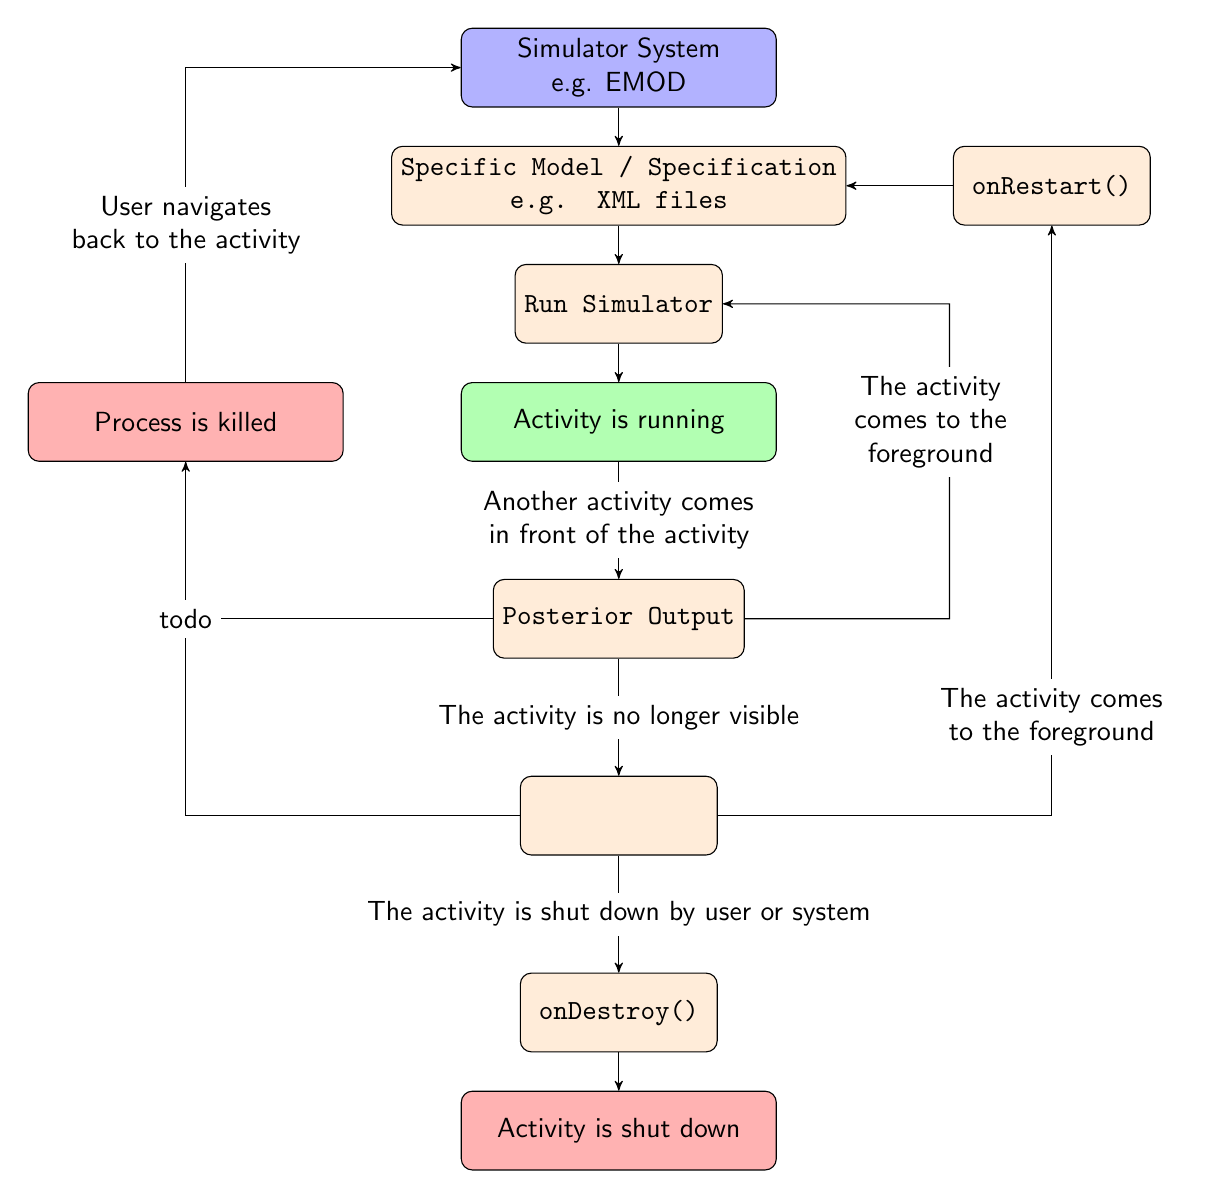
\begin{tikzpicture}[node distance=1.5cm,
    every node/.style={fill=white, font=\sffamily}, align=center]
  % Specification of nodes (position, etc.)
  % \node (start)             [activityStarts]              {Activity starts};
  \node (SimulatorSystem)     [activityStarts]          {Simulator System \\ e.g. EMOD};
  \node (onStartBlock)      [process, below of=SimulatorSystem]   {Specific Model / Specification \\ e.g. XML files};
  \node (onResumeBlock)     [process, below of=onStartBlock]   {Run Simulator};
  \node (activityRuns)      [activityRuns, below of=onResumeBlock]
                                                      {Activity is running};
  \node (onPauseBlock)      [process, below of=activityRuns, yshift=-1cm]
                                                                {Posterior Output};
  \node (onStopBlock)       [process, below of=onPauseBlock, yshift=-1cm]
                                                                 {};
  \node (onDestroyBlock)    [process, below of=onStopBlock, yshift=-1cm] 
                                                              {onDestroy()};
  \node (onRestartBlock)    [process, right of=onStartBlock, xshift=4cm]
                                                              {onRestart()};
  \node (ActivityEnds)      [startstop, left of=activityRuns, xshift=-4cm]
                                                        {Process is killed};
  \node (ActivityDestroyed) [startstop, below of=onDestroyBlock]
                                                    {Activity is shut down};     
  % Specification of lines between nodes specified above
  % with aditional nodes for description 
  % \draw[->]             (start) -- (onCreateBlock);
  \draw[->]     (SimulatorSystem) -- (onStartBlock);
  \draw[->]      (onStartBlock) -- (onResumeBlock);
  \draw[->]     (onResumeBlock) -- (activityRuns);
  \draw[->]      (activityRuns) -- node[text width=4cm]
                                   {Another activity comes in
                                    front of the activity} (onPauseBlock);
  \draw[->]      (onPauseBlock) -- node {The activity is no longer visible}
                                   (onStopBlock);
  \draw[->]       (onStopBlock) -- node {The activity is shut down by
                                   user or system} (onDestroyBlock);
  \draw[->]    (onRestartBlock) -- (onStartBlock);
  \draw[->]       (onStopBlock) -| node[yshift=1.25cm, text width=3cm]
                                   {The activity comes to the foreground}
                                   (onRestartBlock);
  \draw[->]    (onDestroyBlock) -- (ActivityDestroyed);
  \draw[->]      (onPauseBlock) -| node(priorityXMemory)
                                   {todo}
                                   (ActivityEnds);
  \draw           (onStopBlock) -| (priorityXMemory);
  \draw[->]     (ActivityEnds)  |- node [yshift=-2cm, text width=3.1cm]
                                    {User navigates back to the activity}
                                    (SimulatorSystem);
  \draw[->] (onPauseBlock.east) -- ++(2.6,0) -- ++(0,2) -- ++(0,2) --                
     node[xshift=1.2cm,yshift=-1.5cm, text width=2.5cm]
     {The activity comes to the foreground}(onResumeBlock.east);
  \end{tikzpicture}
As stated previously, Simulators are complex systems and should be viewed as black-boxes, thus deciphering the underlying processes occurring within the simulator facilitates the users understanding of how such a system operates and provides a way of interpreting the outputs in a clear way. In addition to this, when using a simulator to make new inferences a user will often want to condition on the output of the simulator, or any new observations gathered. In the standard simulator framework this is not possible, but in 

Essentially, from the users perspective, our approach can be viewed as follows the user would first select the simulator that they are going to use, for example EMOD, they would then write their model, in the desired simulator, according to the given simulator specification. The user would then run the simulator. Now comes the hijacking. During the forward run of the simulator all sampling calls from the random number generator are directed through the probabilistic programming system~(PPS), which in addition to the standard output of the simulator now generates a series of result summaries and path probabilities, as we demonstrate in Section~\ref{sec:casestudy}.

By connecting with the PPS we track all sampling procedures, which enables us to control the myriad of random variables generated within the simulator. 

In order to overhaul a stochastic simulator like EMOD, or OpenMalaria, we are only required to override the location of the stochastic primitives, i.e. the base operations that generate the stochasticity and randomness within the simulator. 
We will walk through how this is done for a standard epidemiology simulator, see the flowchart for a pictorial representation of what is happening \bg{add ref to flow chart}.

The initial step first requires one to build a containerized environment, such as Docker~\cite{merkel2014docker} and Singularity~\cite{kurtzer2017singularity}, which enables the simulators to be run on any device, independent of different hardware architectures, removing the requirement for hardware specific machines. 
This greatly improves the scope of applicability of our system and the simulator, as this environment only has to be built once, which then enables the simulator to be run simultaneously on machines of different architectures machine. This step will be slightly different for individual simulators, but the overall idea is the same. We cannot provide a link to an example of a containerized environment for OpenMalaria and system in this submission due to anonymity\footnote{We shall provide a link in the camera ready submission}.
The second step requires one to override the stochastic primitives, which requires re-writing aspects of the sampling procedures inside the simulator. 
This requires zero domain-expertise and only requires one to find where the sampling calls are originated, this can be done with any basic editor search function.
 Such information is typically saved in $\texttt{RANDOM.<filetype>}$, although it may vary slightly between simulators. We now demonstrate this for a uniform primitive.

% \begin{table}[h!]
% \footnotesize
% \begin{tabular}{p{3.6cm}|p{3.6cm}}
% Before  &  After  \\
% \midrule
% \begin{lstlisting}
% #include <gsl/gsl_cdf.h>
% #include <gsl/gsl_rng.h>
% #include <gsl/gsl_randist.h>
% //preamble
% double random::uniform_01 () {
%     double result =
% # ifdef 
% OM_RANDOM_USE_BOOST
%        rng_uniform01 ();
% # else
%  gsl_rng_uniform (rng.gsl_generator);
% # endif
%     return result;
%     }
% \end{lstlisting}&
% \begin{lstlisting}
% #include <pyprob_cpp.h>
% #include "xtensor/xadapt.hpp"
% // preamble
% double random::uniform_01 () {
% auto uniform = pyprob_cpp::distributions::Uniform(0,1);
% return pyprob_cpp::sample(uniform)(0);
% }
% \end{lstlisting}
% \end{tabular} 
% \end{table}
% As can be seen, writing the new sampling call is cleaner and syntactically simpler. 
The third step is generating the protocols, which enable communication between the simulator and probabilistic programming system. 
For this we extend the existing bridging framework introduced in~\cite{baydin2018efficient}, which is comprised of the Probabilistic Programming eXecution~(PPX) protocols and a light-weight C ++ interface, however the language of this light-weight interface is dependent on whatever the file type of the $\texttt{RANDOM.<filetype>}$ file is. 
For both OpenMalaria and EMOD, the file is written in C ++.
In using these protocols a larger class of sampling procedures can be overridden. The PPX protocols work by making use of the flatbuffer protocols\footnote{\url{https://github.com/google/flatbuffers}}, which require a flatbuffers script to be specified, see here for an example of a flatbuffers script\footnote{https://github.com/probprog/ppx/blob/master/ppx.fbs}. Once this is specified the flat buffers script is compiled and automatically constructs the message passing framework between the simulator and the probabilistic programming system. The flatbuffers script is simple, clean and intuitive, making it easy for a non-expert to produced.
The next steps requires modifying the $\texttt{main}$ function in $\texttt{main.cpp}$ and defining an additional forward function which runs one execution of the simulator to enable message passing between the simulator and PPS\footnote{A link to an example will be provided after the review period to preserve anonymity}.
The final step is to create a light-weight interface. As both the EMOD and OpenMalaria are solely based on C ++ we can extend an existing interface called pyprob\_cpp\footnote{\url{https://github.com/probprog/pyprob_cpp}} to account for the additional sampling procedures.
Once these steps are complete, the containerized environment will now contain everything required to pass models through to the simulators, encode the simulator into a probabilistic program, which can then be evaluated in the PPS.

\bg{Add performance plot showing memory consumptions of pyprob and our new system.}
\section{Case Study}
\label{sec:casestudy}


We provide examples of the generated trace plots from the connection between the simulator and the PPS in Figure~\ref{fig:plotewan}. 
When comparing the two trace plots between EMOD and OgpenMalaria we see significant difference, despite both evaluating the same model for the same disease. 
We can see from the addressing schemes $A_1, \ldots, A_N$ \bg{ref table 1 and 2} what physical events are connected to each other and how outputs in EMOD are generated from a different set of procedures as compared to OpenMalaria 
By having access to such diagrams users can internally evaluate and scrutinize the decisions that the simulator is making.
This is incredibly important for policy makers, or non-experts, as it not only details how we arrive at the given outputs, but it provides an understanding of which processes were most crucial in determining those outputs as can be seen from the path probabilities assigned to each of the vertices.



% 


% \begin{tikzpicture}
% \begin{axis}[xlabel={Population size},ylabel={memory consumption (MB)},
% legend style={at={(0.5,-0.15)},xmin=0,xmax=700,ymin=0,ymax=70, axis lines=center]


% \addplot[pyprob,domain=0:1000, color=blue,]{x};

% \addplot[improved,domain=0:1000, color=red,]{10};

% \legend{pyprob, improved}
% \end{axis}
% \end{tikzpicture}


\begin{figure}
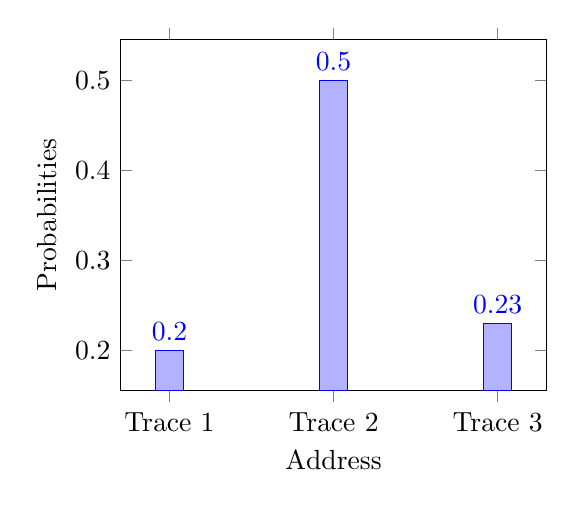
\begin{tikzpicture}
\begin{axis}[
    ybar,
    enlargelimits=0.15,
    legend style={at={(0.5,-0.15)},
      anchor=north,legend columns=-1},
      xlabel = {Address},
    ylabel={Probabilities},
    symbolic x coords={Trace 1, Trace 2, Trace 3},
    xtick=data,
    nodes near coords,
    nodes near coords align={vertical},
    ]
% \addplot coordinates {(tool8,7) (tool9,9) (tool10,4)};
\addplot coordinates {(Trace 1,0.2) (Trace 2,0.5) (Trace 3,0.23)};
% \addplot coordinates {(A1,0.2) (A2,0.5) (A3,0.7) (A4,0.9)};
% \addplot coordinates {(A1,0.1) (A2,0.1) (A3,0.1) (A4,0.3)};
% \legend{used,understood,not understood}
\end{axis}
\end{tikzpicture}
\caption{Trace probabilities. Trace 1 corresponds to A1,A1,A4,... 
Trace 2 corresponds to A1,A1,A1,...A2,... These still need correctly calculating.}
\end{figure}
\begin{figure*}[h!]
	\centering
	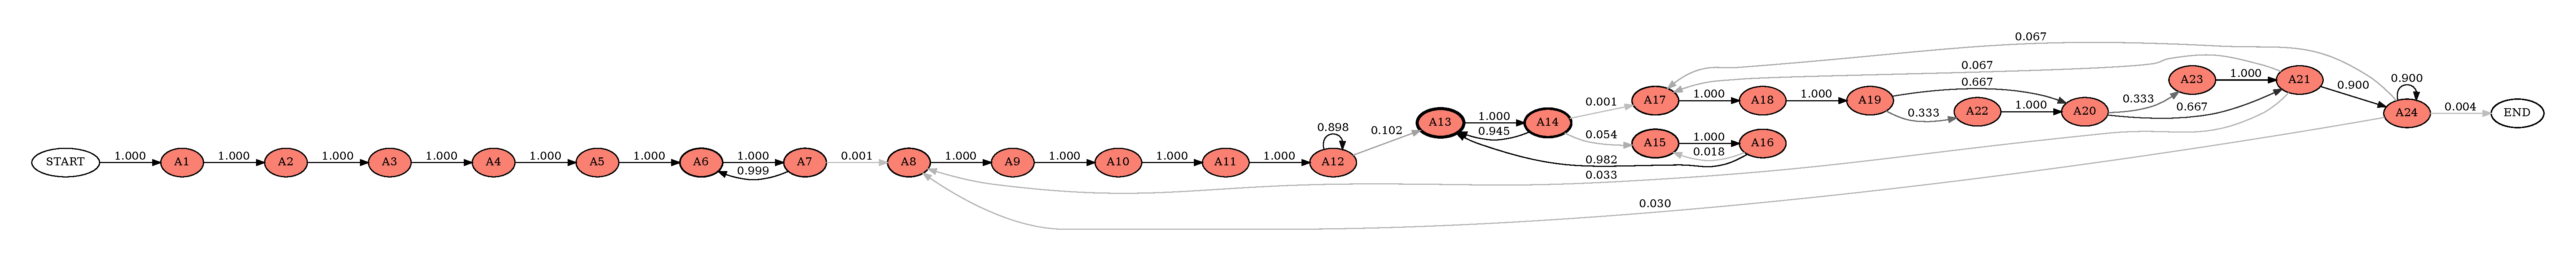
\includegraphics[width=\textwidth]{../plots/emod_24_prior_pop_100.pdf}
	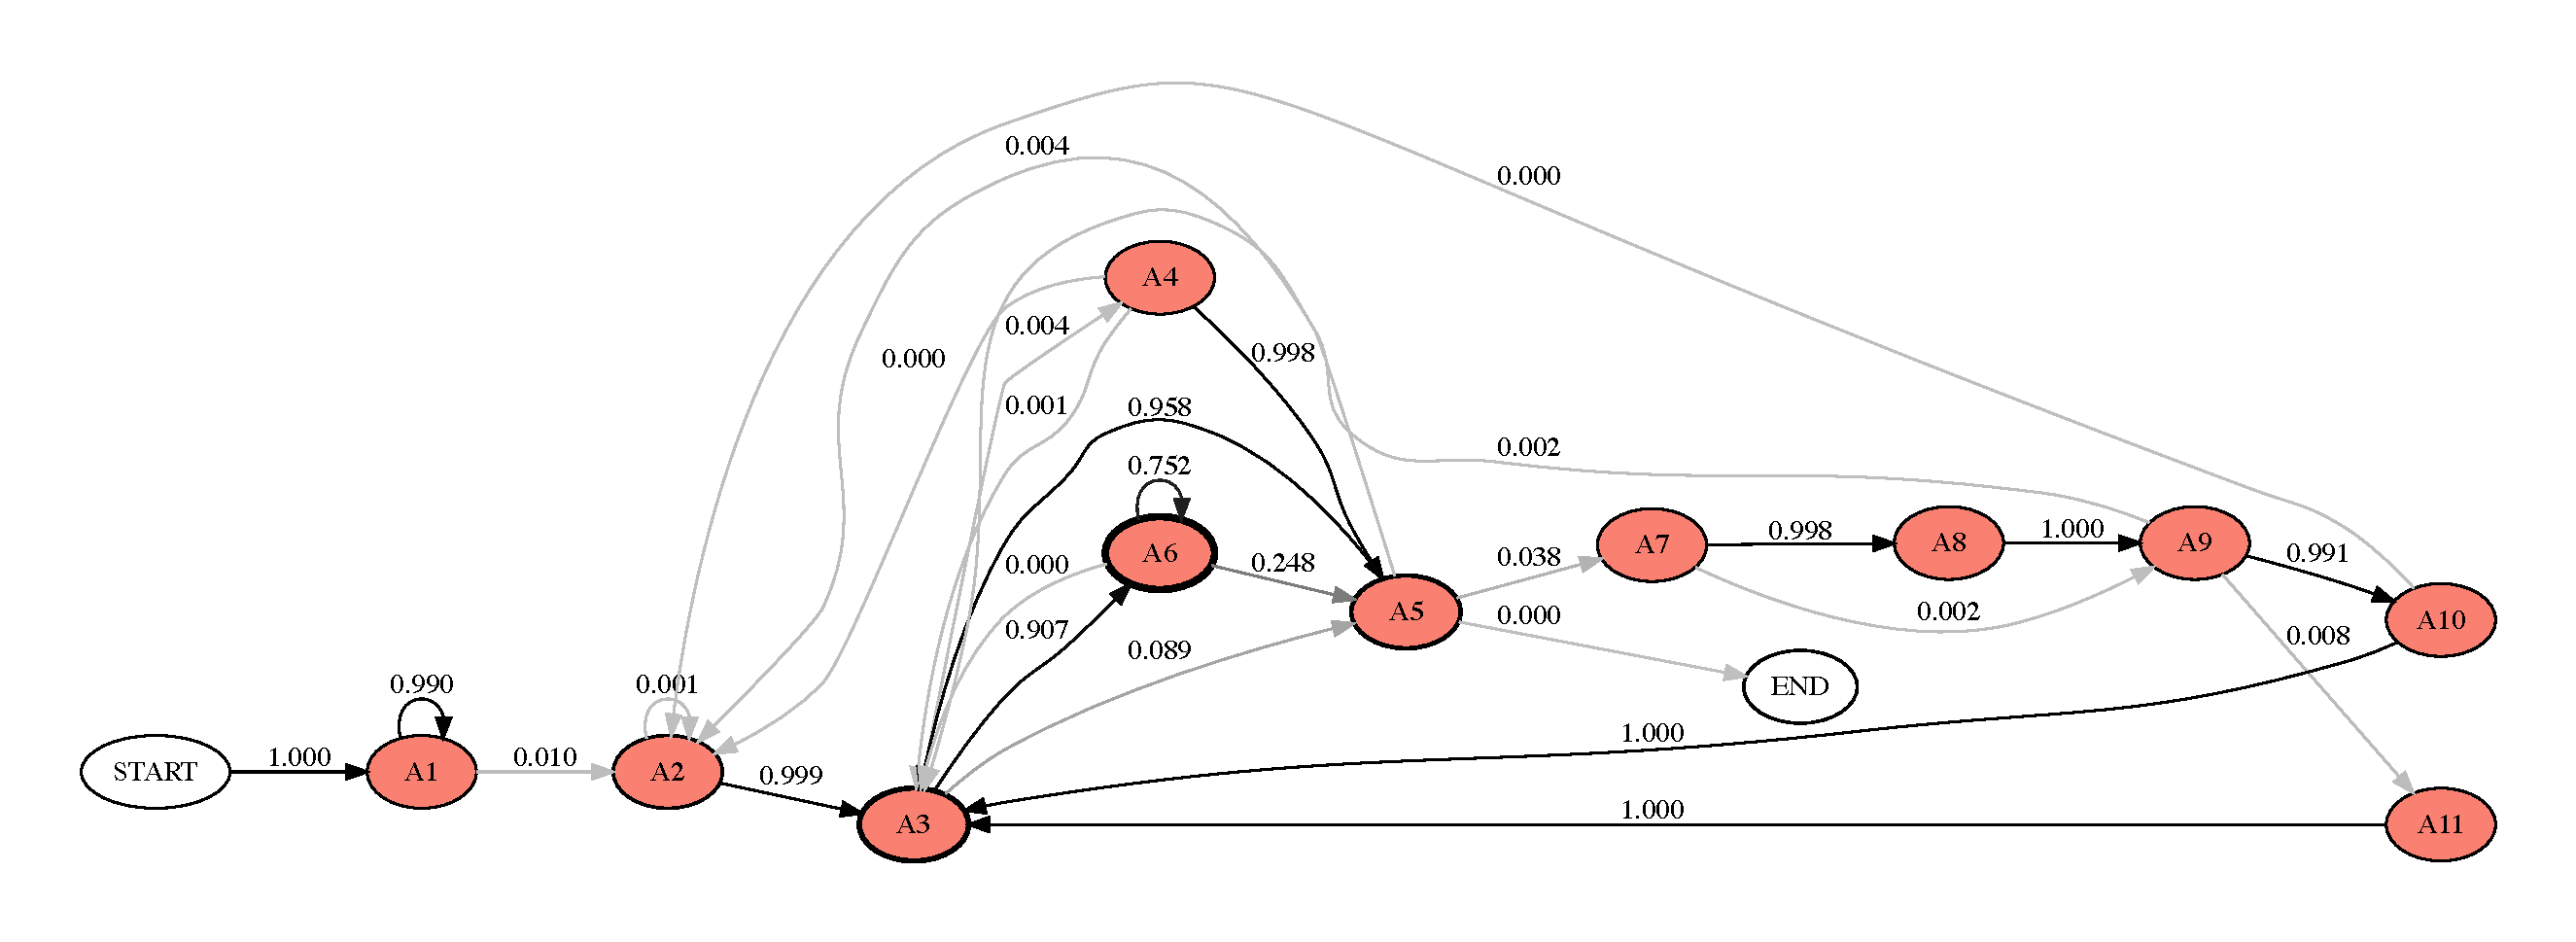
\includegraphics[width=\textwidth]{../plots/ewan_25_pop_100.pdf}
	\caption{Here we run two equivalent models, compare the corresponding trace paths and corresponding 
	path probabilities taken by the thousands of random variables generated internally within the simulators. \textit{\textbf{Top:}} The specified model run in EMOD. \textit{\textbf{Bottom:}} The specified model in OpenMalaria.}
	\label{fig:plotewan}
\end{figure*}

 \begin{table*}[h!]
  \footnotesize
  \setlength{\tabcolsep}{1mm}
  \caption{A few addresses generated for the OpenMalaria simulator, see the Supplement for the full table.}
  \label{table:addresses}
  \def\arraystretch{1.25}
  % \setlength{\tabcolsep}{1mm}
  \begin{tabularx}{\textwidth}{@{}lX@{}} 
    \toprule
    Address ID & Full address \\
    \midrule
  A1 & [forward()+0x204; OM::Simulator::start(scnXml::Monitoring const)+0x28a;

  OM::Population::createInitialHumans()+0x94;

  OM::Population::newHuman(OM::SimTime)+0x5c;

  OM::Host::Human::Human(OM::SimTime)+0x12b;

  OM::WithinHost::WHInterface::createWithinHostModel(double)+0x99;

  OM::WithinHost::DescriptiveWithinHostModel::DescriptiveWithinHostModel(double)+0x3a;

  OM::WithinHost::WHFalciparum::WHFalciparum(double)+0xe6;

  OM::util::random::gauss(double, double)+0xb4]\_\_Normal\\

   $\vdots$ & $\vdots$ \\
  A5 & [forward()+0x204; OM::Simulator::start(scnXml::Monitoring const\&)+0x468;

   OM::Population::update1(OM::SimTime)+0xff;

    OM::Host::Human::update(bool)+0x2bc;

    OM::Clinical::ClinicalModel::update(OM::Host::Human\&, double, bool)+0x96;

    OM::Host::NeonatalMortality::eventNeonatalMortality()+0x9;

    OM::util::random::uniform\_01()+0xc0]\_\_Uniform\\


 $\vdots$ & $\vdots$ \\

\bottomrule
  \end{tabularx}
  \end{table*}

\bibliographystyle{icml2019}
\bibliography{malaria,refs}


\end{document}


% This document was modified from the file originally made available by
% Pat Langley and Andrea Danyluk for ICML-2K. This version was created
% by Iain Murray in 2018, and modified by Alexandre Bouchard in
% 2019. Previous contributors include Dan Roy, Lise Getoor and Tobias
% Scheffer, which was slightly modified from the 2010 version by
% Thorsten Joachims & Johannes Fuernkranz, slightly modified from the
% 2009 version by Kiri Wagstaff and Sam Roweis's 2008 version, which is
% slightly modified from Prasad Tadepalli's 2007 version which is a
% lightly changed version of the previous year's version by Andrew
% Moore, which was in turn edited from those of Kristian Kersting and
% Codrina Lauth. Alex Smola contributed to the algorithmic style files.
